% =====================================================================================
%  AIoT energy anomaly detection — IEEE conference manuscript
%
%  BUILD:  python scripts/build_paper.py     (copies figures, then runs pdflatex twice)
%  Every number in this file is produced by a script under src/ and stored in
%  results/metrics/*.json. tests/test_paper_numbers.py fails if they drift apart.
% =====================================================================================
\documentclass[conference]{IEEEtran}

\usepackage{amsmath}
\usepackage{booktabs}
\usepackage{graphicx}
\usepackage{url}
\usepackage[hidelinks]{hyperref}
\usepackage{siunitx}

\graphicspath{{figures/}}

\newcommand{\simnote}{\textbf{SIMULATED}}

\begin{document}

\title{Causal, Building-Disjoint Anomaly Detection for Hourly Energy Telemetry:\\
An XGBoost Pipeline, Its Failure Modes, and a Transfer Test to Simulated\\
Geothermal Auxiliary Equipment}

\author{
\IEEEauthorblockN{AIoT Research Agent}
\IEEEauthorblockA{Autonomous research pipeline \\
Project: \texttt{E:\textbackslash project\textbackslash LAB\_AI\textbackslash AIoT} \\
\textit{Manuscript generated from reproducible artefacts}}
}

\maketitle

\begin{abstract}
Condition monitoring of geothermal power-plant auxiliary equipment requires detecting rare faults in
dense, strongly autocorrelated telemetry, and it is usually attempted with no labelled faults from the
plant itself. We report a complete, reproducible study of that setting on a public dataset with real
human annotations: 1{,}749{,}494 hourly electricity readings from 200 commercial buildings
(LEAD1.0-small), of which 2.13\% are anomalous. We make four contributions. First, we formalise a
\emph{causal feature contract} --- every feature at time $t$ is a function of readings at times
$\le t$ only --- and enforce it with an executable truncation test rather than by review; median
lag-one autocorrelation is 0.933, so the contract is what separates a real result from a leaked one.
Second, we evaluate with a building-disjoint protocol (140/30/30) that mimics deployment on an
uninstrumented asset. Third, an XGBoost model over 34 causal features reaches ROC-AUC
0.9524 (95\% CI 0.9249--0.9702), PR-AUC 0.8342 against a 2.24\% base rate, and detects 82.3\% of
anomaly episodes with a median latency of one hour at 0.056 false-alarm episodes per building-day,
while remaining calibrated (ECE 0.0005). Fourth, we report the parts that usually go unpublished: a
family ablation showing that simple dynamics features alone reach 0.928 ROC-AUC, a class-weighting
experiment that triples the Brier score for 1.6 points of episode recall, a per-building recall range
of 0.02--1.00, and a transfer test to \simnote{} geothermal signals in which the frozen operating
threshold flags 0 of 252 injected fault hours. The last result is the most useful one for practice:
a threshold calibrated on one asset population does not transfer, and anomaly detectors for
industrial equipment must be recalibrated per asset.
\end{abstract}

\begin{IEEEkeywords}
anomaly detection, industrial IoT, condition monitoring, XGBoost, SHAP, reproducibility,
class imbalance, geothermal power plant, LEAD1.0
\end{IEEEkeywords}

\section{Introduction}

Geothermal power plants are monitored by dense instrumentation: circulating-water pumps, non-condensable
gas (NCG) extraction compressors, separator level control, and turbine bearing temperatures all stream
hourly or faster. Faults are rare, expensive, and often preceded by hours or days of subtle drift.
The practical question is not ``is this reading high?'' but ``is this reading unusual \emph{for this
asset, right now}?'' --- which is a question about a residual, not a magnitude.

Two difficulties dominate. The first is \emph{label scarcity}: a plant accumulates perhaps a handful of
confirmed faults per year, so supervised detection is usually impossible and practitioners fall back on
unsupervised outlier scores or static limits. The second is \emph{temporal leakage}: telemetry is
strongly autocorrelated, so any evaluation that splits rows at random will reward a model for reading
the neighbouring hour. On the dataset used here, median lag-one autocorrelation is 0.933 and median
lag-24 h autocorrelation is 0.681; a row-wise split is therefore not a weak evaluation but a
meaningless one.

This paper reports a study designed around those two difficulties. We use a public dataset that has
real, human-produced anomaly annotations (LEAD1.0-small, derived from the ASHRAE Great Energy
Predictor III readings), which lets us study supervised detection without pretending that labels exist
where they do not. We then evaluate in a way that matches the deployment question --- \emph{will this
catch faults in a building the model has never seen?} --- and we report what fails.

\subsection*{Contributions}

\begin{enumerate}
\item A \emph{causal feature contract} with an executable test: features are rebuilt on history
truncated at $T$ and must be bit-identical at $t \le T$. This turns leakage from a review opinion into
a failing assertion (Section~\ref{sec:method}).
\item A building-disjoint evaluation protocol, fixed before any model was trained, with
label-rate-balanced assignment and a building-level bootstrap for uncertainty.
\item A measured account of what carries the signal: dynamics features alone reach 0.928 ROC-AUC,
while calendar features reach 0.729 ROC-AUC but 0.064 PR-AUC --- i.e.\ they rank rows without
identifying anomalies (Section~\ref{sec:results}).
\item An evaluation that separates \emph{point} detection from \emph{episode} detection, and a
per-building breakdown that exposes a bimodal distribution hidden by the aggregate AUC.
\item A deployment artefact (FastAPI service plus dashboard) in which serving and training share one
feature builder, verified to $10^{-6}$, and a transfer test on \simnote{} geothermal signals that
fails in an informative way.
\end{enumerate}

\subsection*{What this paper does not claim}

The model is trained on commercial-building electricity, not on a geothermal plant. No PLTP Kamojang
measurement was available, and none is reported. All geothermal signals in this work are
\simnote{}; the transfer experiment in Section~\ref{sec:transfer} measures the behaviour of the
pipeline on synthetic data and says nothing about plant performance. We also do not compare our
numbers with published LEAD1.0 benchmarks, because those use the competition split and metrics that
we could not reproduce in this environment.

\section{Related Work}

\emph{Anomaly detection.} Chandola \emph{et al.}~\cite{chandola2009} organise the field into
statistical, proximity-based and classification-based families; our setting is the classification case
with extreme imbalance and temporal dependence. Isolation Forest~\cite{liu2008} is the standard
label-free baseline and is included here, and it illustrates the central limitation: it ranks gross
outliers well but detects only 30\% of anomalies at a 1\% false-positive rate.

\emph{Gradient boosting and explanations.} XGBoost~\cite{chen2016} remains the default tabular model,
and its native handling of missing values matters here because 6.15\% of readings are absent. We use
SHAP~\cite{lundberg2017} to attribute the score, and we report it alongside gain importance because the
two rank features differently: gain measures split usefulness, SHAP measures effect on the output.

\emph{Metrics.} ROC analysis~\cite{fawcett2006} is insensitive to prevalence; for rare anomalies the
precision--recall view~\cite{saito2015} is more informative, so both are reported. We additionally
report \emph{episode-level} recall, since a six-hour fault that is flagged once has been detected, and
point-wise metrics cannot express that.

\emph{Validation with dependence.} Bergmeir \emph{et al.}~\cite{bergmeir2018} and
Roberts \emph{et al.}~\cite{roberts2017} show that naive cross-validation is invalid under temporal and
hierarchical dependence. Our response is group-disjoint splitting by building, which removes the
within-asset dependence entirely.

\emph{Datasets.} LEAD1.0~\cite{gulati2022} contributes the annotations used here; the underlying
readings come from the ASHRAE Great Energy Predictor III competition~\cite{miller2020}.

\section{Data and Problem Formulation}
\label{sec:data}

\subsection{Dataset}

LEAD1.0-small contains 1{,}749{,}494 rows over 200 buildings and 8{,}784 hourly timestamps
(2016-01-01 to 2016-12-31), with a binary anomaly annotation per (building, hour). Table~\ref{tab:audit}
summarises the audit, produced by \texttt{src/data/audit.py}.

\begin{table}[t]
\centering
\caption{Dataset audit. All values are produced by \texttt{src/data/audit.py}.}
\label{tab:audit}
\begin{tabular}{lr}
\toprule
Rows & 1{,}749{,}494 \\
Buildings & 200 \\
Hourly timestamps & 8{,}784 \\
Anomalous hours & 37{,}296 (2.13\%) \\
Imbalance ratio & 45.91 : 1 \\
Missing \texttt{meter\_reading} & 107{,}653 (6.15\%) \\
Anomaly episodes & 5{,}503 \\
Median episode length & 2 h \\
Single-hour episodes & 47.2\% \\
Median lag-1 autocorrelation & 0.933 \\
Median lag-24 h autocorrelation & 0.681 \\
\bottomrule
\end{tabular}
\end{table}

Two properties drive every later design decision. The annotation is \emph{episodic}: 5{,}503
contiguous events with median length 2 h, half of them single hours. And the labels are
\emph{incomplete by construction} at missing hours --- none of the 107{,}653 hours without a reading
carries a positive label, because there is nothing to annotate.

\subsection{Problem statement}

For each row $i$ with building $b(i)$, timestamp $t_i$ and reading $x_i$, predict
$p_i = P(y_i = 1 \mid \mathcal{H}_{b(i), \le t_i})$, where $\mathcal{H}$ is the asset's own history.
The model never sees $b(i)$ as an input: under a building-disjoint protocol an identifier cannot
generalise, and including it would silently convert the task into per-building memorisation.

\subsection{Splits}

Buildings are sorted by their per-building anomaly rate and assigned greedily to whichever split is
furthest behind its target share (140 train / 30 validation / 30 test). Sorting before assignment keeps
the label rate balanced: 2.162\%, 2.049\% and 2.072\% respectively. The training buildings are further
partitioned into five grouped folds of 28 for hyper-parameter selection. The test split was scored once,
after the model and its threshold were frozen.

\subsection{Handling of missing readings}
\label{sec:missing}

Because a missing hour is never labelled anomalous, a model trained on all rows learns the
deterministic rule ``missing $\Rightarrow$ normal''. That rule is worth 6.15\% of the data for free and
is operationally wrong: a dead sensor is a fault. We therefore drop unobserved rows from training and
from all reported metrics (measured effect on ROC-AUC: 0.9576 $\rightarrow$ 0.9554), and the serving
layer reports such hours as a distinct \textsc{Outage} alarm. The anomaly prevalence on observed rows,
2.27\%, differs from the dataset-wide 2.13\% and the two are never mixed.

\section{Method}
\label{sec:method}

\subsection{Causal feature contract}

\begin{quote}
Every feature value at time $t$ is a deterministic function of
$\{(b, x_s) : s \le t\}$ for the same asset, and of nothing else.
\end{quote}

Three consequences are enforced in code. (i) All rolling statistics are computed on
\texttt{series.shift(1)}, so the current reading never enters its own baseline. (ii) Each building is
reindexed onto the full hourly grid before windowing, so a 24-row window always spans 24 hours even
where source rows are absent; absent hours are not re-emitted as training rows. (iii) No feature may
depend on another asset. The third rule was adopted after it was violated: an earlier cross-sectional
``peer'' feature could not be reproduced at single-asset inference time and produced a 57\%
train/serve discrepancy, which the serving test caught. Removing it did not hurt
(validation ROC-AUC 0.9539 $\rightarrow$ 0.9543).

The contract is verified empirically, not asserted. \texttt{tests/test\_features\_no\_leakage.py}
rebuilds the feature matrix on history truncated at $T$ and requires every value at $t \le T$ to be
identical to the full-history build; a second test perturbs only the reading at $t$ and requires the
past-only baselines to be unchanged. Any centred window, negative shift or forward fill fails
immediately.

\subsection{Features}

34 features in six families (Table~\ref{tab:features}). Only scale-free transforms of the level are
used, because building medians span 57--969\,kWh and a raw magnitude does not transfer across assets.

\begin{table}[t]
\centering
\caption{Feature families (34 features). Windows are 6, 24, 168 and 720 hours with
\texttt{min\_periods} 3, 12, 24 and 48.}
\label{tab:features}
\small
\begin{tabular}{llr}
\toprule
Family & Examples & $n$ \\
\midrule
level & $\log(1+x)$, $x/\mathrm{median}_{w}$ & 5 \\
deviation & $(x-\mu_w)/\sigma_w$, $(x-\mu_w)/\mu_w$ & 8 \\
dynamics & $\Delta x$, $x-x_{t-24}$, $x-x_{t-168}$, momentum & 9 \\
volatility & $\sigma_w/\mu_w$, $(\max_w-\min_w)/\mu_w$ & 4 \\
availability & hours since last reading, missing count in 24 h & 3 \\
calendar & hour/dow sine-cosine, month, weekend & 6 \\
\bottomrule
\end{tabular}
\end{table}

\subsection{Model and metrics}

XGBoost~\cite{chen2016} with histogram splits, depth 8, learning rate 0.03, $\lambda=5$,
$\alpha=0.1$, subsample 0.9, column sample 0.6, early stopping (75 rounds) on validation PR-AUC;
734 trees. The class prior is left intact: predicted probabilities are then comparable with the cost
of an inspection, which matters for a dashboard that shows a number to an operator.

The operating threshold maximises $F_2$ on validation (recall weighted twice precision, matching the
cost asymmetry of missed incipient faults) and is frozen before test. Reported metrics: ROC-AUC and
PR-AUC (threshold-free), Brier score and expected calibration error, recall at 1\% and 0.1\% false
positive rate, and episode-level recall with detection latency. Uncertainty is a building-level
bootstrap (300 resamples) --- resampling rows would ignore the clustering that the protocol creates.

\subsection{Hyper-parameter search}

A capped TPE search was attempted and abandoned: each trial cost about 100\,s, and a resumed study
replayed identical parameter sets because the sampler restarts its seeded random phase on reload. A
deterministic six-candidate grid replaced it (two grouped folds, 20\% row subsample). All six
candidates fell within 0.0026 PR-AUC of each other, so hyper-parameters are not the lever here;
features and labels are. The best candidate was selected by validation ROC-AUC and frozen.

\section{Results}
\label{sec:results}

\subsection{Baselines and model}

\begin{table}[t]
\centering
\caption{Validation split (30 buildings, 250{,}019 observed rows). Threshold-dependent columns are at
the $F_2$-optimal threshold for each model.}
\label{tab:val}
\small
\begin{tabular}{lcccc}
\toprule
Model & ROC-AUC & PR-AUC & Brier & Episode rec. \\
\midrule
Prior (constant) & 0.5000 & 0.0215 & 0.0210 & --- \\
Isolation Forest & 0.8058 & 0.2296 & 0.1348 & 0.474 \\
Logistic regression & 0.8087 & 0.5715 & 0.0130 & 0.780 \\
XGBoost (selected) & \textbf{0.9562} & \textbf{0.8198} & \textbf{0.0066} & \textbf{0.896} \\
\bottomrule
\end{tabular}
\end{table}

Table~\ref{tab:val} establishes three things. The problem is learnable from telemetry alone: a linear
model on the same features reaches 0.809 ROC-AUC, so the signal is not an artefact of tree
flexibility. Annotations are worth a great deal: the label-free Isolation Forest ranks reasonably
(0.806 ROC-AUC) but its PR-AUC (0.230) and 1\%-FPR recall (0.301) show that it cannot identify
anomalies at a workable alert rate. And gradient boosting adds roughly 0.15 ROC-AUC over the linear
model, i.e.\ the interactions matter.

\subsection{What carries the signal}

\begin{table}[t]
\centering
\caption{Family-only ablation, validation split. Each row is a model trained on one family.}
\label{tab:ablation}
\small
\begin{tabular}{lcccc}
\toprule
Family & $n$ & ROC-AUC & PR-AUC & Episode rec. \\
\midrule
dynamics & 9 & \textbf{0.9284} & \textbf{0.7657} & \textbf{0.881} \\
deviation & 8 & 0.9072 & 0.7268 & 0.581 \\
level & 5 & 0.9011 & 0.6734 & 0.431 \\
volatility & 4 & 0.8290 & 0.4507 & 0.362 \\
calendar & 6 & 0.7290 & 0.0640 & 0.337 \\
availability & 2 & 0.6492 & 0.0870 & 0.543 \\
\midrule
all & 34 & 0.9562 & 0.8198 & 0.896 \\
\bottomrule
\end{tabular}
\end{table}

Table~\ref{tab:ablation} is the most transferable finding in this paper. \emph{Dynamics} features ---
first differences, same-hour-yesterday and same-hour-last-week comparisons, short-versus-long
momentum --- reach 0.928 ROC-AUC on their own and, at 0.881, essentially match the full model's episode
recall. Anomalies in this data are \emph{changes}, not \emph{levels}. Level features alone score 0.901
ROC-AUC but only 0.431 episode recall: they fire on the peak hour of an episode and miss the rest,
which is precisely the gap that point-wise metrics hide. Calendar features rank rows at 0.729 ROC-AUC
yet achieve 0.064 PR-AUC --- they carry no anomaly information, only the base-rate shape of the day.
Availability features, i.e.\ past outages, reach 0.649 ROC-AUC, confirming that sensor dropouts precede
annotated anomalies.

\subsection{Class weighting, measured}

\begin{table}[t]
\centering
\caption{Effect of \texttt{scale\_pos\_weight} = 42.4 on the validation split.}
\label{tab:weight}
\small
\begin{tabular}{lcccc}
\toprule
 & ROC-AUC & PR-AUC & Brier & Episode rec. \\
\midrule
unweighted (selected) & \textbf{0.9562} & \textbf{0.8198} & \textbf{0.0066} & 0.896 \\
weighted & 0.9519 & 0.8182 & 0.0234 & \textbf{0.912} \\
\bottomrule
\end{tabular}
\end{table}

The standard reflex for 43:1 imbalance is to reweight the positive class. Table~\ref{tab:weight} shows
what that buys: 1.6 points of episode recall, at the cost of 0.4 points of ROC-AUC, 0.2 points of
PR-AUC, and a Brier score 3.5 times worse. Since the deployment displays probabilities to an operator
and moves the operating point instead, the unweighted model is retained.

\subsection{Held-out performance}

The test split (30 unseen buildings, 243{,}684 observed rows, 5{,}454 anomalies) was scored once.

\begin{table}[t]
\centering
\caption{Held-out test performance of the frozen model.}
\label{tab:test}
\small
\begin{tabular}{lr}
\toprule
ROC-AUC (95\% CI) & 0.9524 (0.9249--0.9702) \\
PR-AUC (base rate 0.0224) & 0.8342 \\
Brier / ECE (12 quantile bins) & 0.00613 / 0.0005 \\
Recall at FPR $=1\%$ / $0.1\%$ & 0.8089 / 0.7329 \\
Precision / recall at $\tau=0.1283$ & 0.7987 / 0.7888 \\
Alert rate & 2.21\% of hours \\
Anomaly episodes & 536 \\
Episodes detected (recall) & 441 (0.8228) \\
Median detection latency & 1 h \\
False-alarm episodes per building-day & 0.056 \\
Median per-building recall & 0.842 \\
\bottomrule
\end{tabular}
\end{table}

Fig.~\ref{fig:rocpr} and Table~\ref{tab:test} give the headline: ROC-AUC 0.9524 with a building-level
95\% interval of 0.9249--0.9702, PR-AUC 0.8342 against a 2.24\% base rate, and 82.3\% of episodes
detected with a one-hour median latency and 0.056 false-alarm episodes per building-day. Calibration is
essentially exact (ECE 0.0005 over predicted probabilities spanning $3\times10^{-4}$ to $0.3$,
Fig.~\ref{fig:calib}), which is a direct consequence of leaving the prior intact.

\begin{figure}[t]
\centering
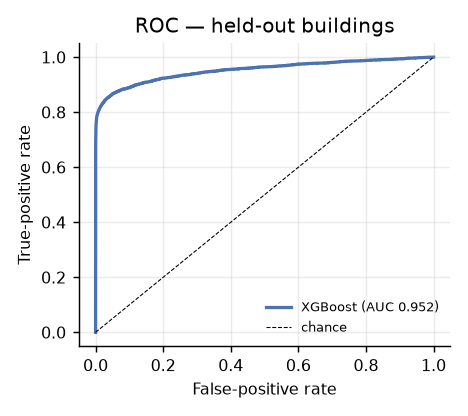
\includegraphics[width=0.48\linewidth]{holdout_roc_final.png}
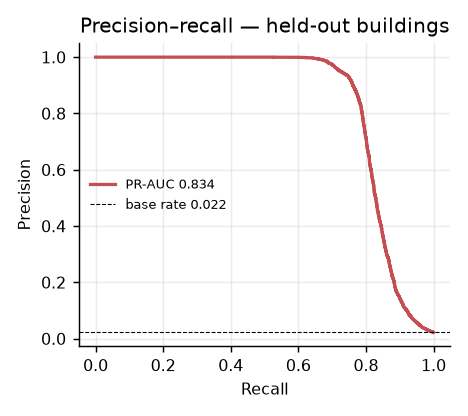
\includegraphics[width=0.48\linewidth]{holdout_pr_final.png}
\caption{Left: ROC on 30 held-out buildings. Right: precision--recall with the base rate as reference.
Both from \texttt{src/evaluation/holdout.py}.}
\label{fig:rocpr}
\end{figure}

\begin{figure}[t]
\centering
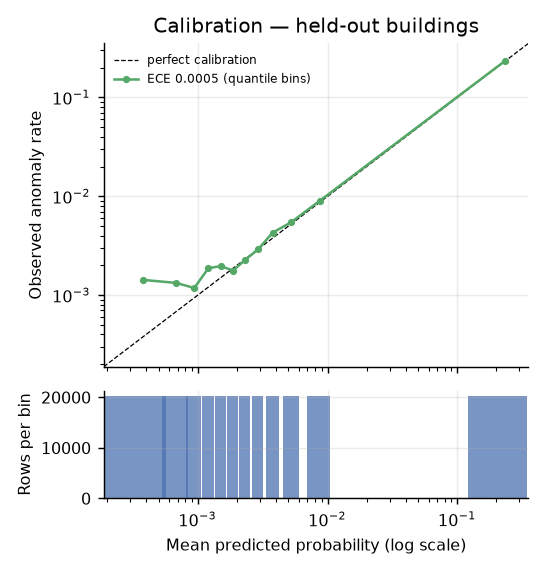
\includegraphics[width=0.78\linewidth]{holdout_calibration_final.png}
\caption{Reliability of predicted probabilities on held-out buildings (log--log), with the number of
rows per bin below. ECE $=0.0005$. Equal-width binning is not used: with a 2.2\% prevalence it
collapses every prediction into one bin.}
\label{fig:calib}
\end{figure}

\subsection{Per-asset heterogeneity}

The aggregate AUC conceals a bimodal distribution. Per-building recall has median 0.842, with 8 of 30
buildings above 0.9 and 4 below 0.5; the worst building catches 1 of 58 anomalies (recall 0.017,
mean score 0.009). These are buildings whose annotated anomalies are small relative to their own
volatility --- an intrinsic property of self-referential detection: an excursion of 20\% in a noisy
asset is indistinguishable from normal operation. The practical implication is that per-asset recall
must be reported and monitored, which the deployed service does.

\subsection{Feature attribution}

\begin{figure}[t]
\centering
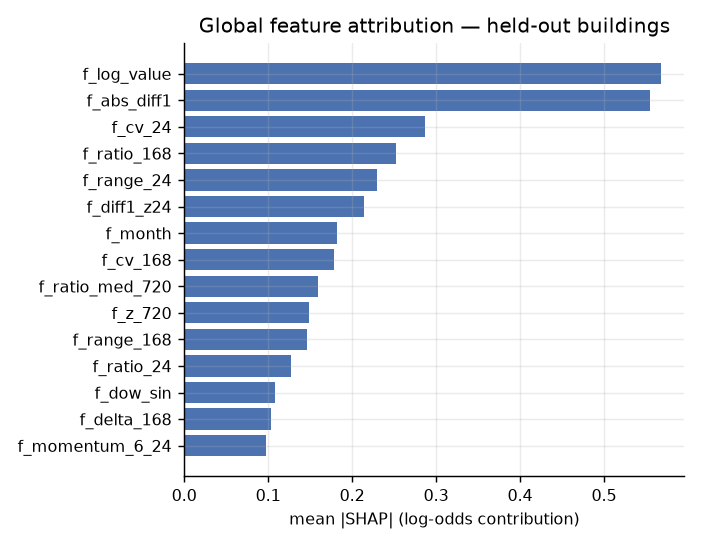
\includegraphics[width=0.62\linewidth]{shap_global_final.png}
\caption{Mean $|$SHAP$|$ over a uniform random sample of the test split (deployment prevalence),
computed with TreeExplainer.}
\label{fig:shap}
\end{figure}

On the deployment distribution (Fig.~\ref{fig:shap}), the strongest contributors are the log level
(0.567), the absolute hour-to-hour difference (0.554), the 24-hour coefficient of variation (0.287),
the ratio to the 7-day mean (0.252) and the 24-hour range (0.230). Gain importance instead ranks
\texttt{dev\_rel\_720} and \texttt{abs\_diff1} first; the two measures answer different questions and
are both reported. We note explicitly that SHAP magnitudes depend on the sample distribution --- an
earlier run that oversampled anomalies by 5$\times$ reordered the top features --- so the sampling is
stated with the figure.

\section{Deployment}
\label{sec:deploy}

\subsection{One scoring path}

A FastAPI service exposes the frozen model (\texttt{/model}, \texttt{/metrics}), held-out series
(\texttt{/buildings}, \texttt{/buildings/\{id\}/series}), single-asset scoring (\texttt{/score}) and
batch scoring (\texttt{/batch}). The critical property is that serving calls the \emph{same}
\texttt{build\_feature\_frame} used to construct the training matrix, on the caller's history. A test
scores a real row through both paths and requires agreement to $10^{-6}$; this is what caught the
cross-asset feature described in Section~\ref{sec:method}.

Alarms are typed: \textsc{Anomaly} (score above threshold), \textsc{Normal}, and \textsc{Outage} (no
reading). Outages are never scored, because the labels cannot describe them and because conflating a
dead sensor with a consumption anomaly would hide the more urgent fault.

\subsection{Interactive dashboard}

A dependency-free page (no build step, no CDN) renders the KPI strip, a held-out building explorer
with readings, annotations and flagged hours, and a threshold slider that recomputes precision and
recall for the selected asset. It defaults to the median-performing building and labels each option
with its recall, so that the per-asset spread is visible on first load rather than buried.

\subsection{Transfer test on \simnote{} geothermal signals}
\label{sec:transfer}

We generated 90 days of hourly signals for four auxiliary systems (cooling-water pump power, NCG
compressor current, turbine bearing temperature, separator level) with four injected faults of known
extent, and scored them with the frozen building-trained model. Every output is tagged
\textbf{SIMULATED}; these are not plant measurements and the exercise is a pipeline test, not a
performance claim.

\begin{table}[t]
\centering
\caption{Transfer to \simnote{} geothermal signals at the frozen building threshold.}
\label{tab:sim}
\small
\begin{tabular}{lccr}
\toprule
Signal (injected fault) & ROC-AUC & PR-AUC & Fault hours flagged \\
\midrule
separator level (drift) & 0.954 & 0.110 & 0 / 24 \\
pump power (cavitation) & 0.868 & 0.142 & 0 / 36 \\
bearing temp.\ (overheat) & 0.579 & 0.094 & 0 / 72 \\
compressor current (fouling) & 0.389 & 0.042 & 0 / 120 \\
\bottomrule
\end{tabular}
\end{table}

The result (Table~\ref{tab:sim}) is a failure, and a useful one. Zero of 252 fault hours are flagged:
scores on these signals sit an order of magnitude below the building-calibrated threshold, so the alarm
never fires even where the ranking is good (separator: ROC-AUC 0.954, no alarms). Ranking itself
transfers only partially --- well for a slow drift, badly for compressor fouling, whose ramp is small
relative to that signal's own noise. The lesson is direct: an absolute operating threshold is only
valid for the population on which it was calibrated, and cross-asset deployment requires
recalibration at minimum and retraining in practice. We deliberately did not tune anything on the
simulation.

\section{Discussion}

\emph{Why dynamics dominate.} Anomalies in annotated commercial-building data are predominantly step
changes and spikes relative to an asset's own baseline. A detector built on ratios to recent history
therefore generalises across assets with medians differing by an order of magnitude, while a detector
built on absolute levels does not. The same argument applies to rotating machinery, where the
informative signal is usually a residual against a learned baseline rather than an absolute value.

\emph{Why the threshold is the fragile part.} The model's ranking transfers better than its
calibration: PR-AUC 0.097 on simulated signals is poor, but the separator reaches 0.954 ROC-AUC while
producing no alarms at all. Any deployment that hard-codes a probability threshold inherits the
calibration of its training population. Per-asset thresholding on a held-out period of that asset's
own data is the minimum viable remedy.

\emph{Labels are the binding constraint.} The gap between the Isolation Forest (0.230 PR-AUC) and the
supervised model (0.820) is the value of annotation. For a geothermal plant, that argues for
structuring maintenance records into labelled episodes --- a process change, not a modelling one.

\section{Threats to Validity}

\begin{itemize}
\item \emph{Label noise.} LEAD1.0 annotations are human/rule-assisted; some labelled anomalies are
benign operating changes. No second annotator exists, so this is stated rather than quantified.
\item \emph{Domain.} All 200 assets are commercial buildings in one year and one climate. Transfer to
geothermal equipment is untested; the simulation is a pipeline demonstration only.
\item \emph{Single split.} The split is deterministic and was not repeated. The building-level
bootstrap CI partially covers this, and the hyper-parameter surface was shown to be flat, so the
conclusions do not hinge on the draw.
\item \emph{Threshold transfer.} The $F_2$ threshold is calibrated to a 2.2\% prevalence; a plant with
a different anomaly rate must re-derive it. The service exposes the threshold as configuration.
\item \emph{Incomparable benchmarks.} The Kaggle competition split for LEAD1.0 was unavailable (no
credentials, no mirror), so no published score is quoted alongside ours.
\end{itemize}

\section{Reproducibility}

The repository contains every stage as a runnable module: audit, EDA, feature build, split,
baselines, tuning grid, training, selection, holdout evaluation, SHAP, simulation, API and dashboard.
Dataset acquisition is pinned by URL and SHA-256 and re-verified on download. Dependencies are pinned
to exact versions (Python 3.14.9, \texttt{numpy} 2.5.4, \texttt{pandas} 3.1.1, \texttt{scikit-learn}
1.9.1, \texttt{xgboost} 3.4.1, \texttt{shap} 0.54.1). Every reported number is written to
\texttt{results/metrics/*.json} by the script that computes it, and
\texttt{tests/test\_paper\_numbers.py} fails if a headline value in this manuscript diverges from
those files. The test suite comprises 33 tests, including the leakage truncation test, the
serving/batch agreement test and the API contract tests.

\section{Conclusion}

We reported a complete, reproducible anomaly-detection pipeline for hourly energy telemetry, evaluated
on assets the model has never seen: ROC-AUC 0.9524, PR-AUC 0.8342, 82.3\% episode recall at one-hour
median latency, and calibrated probabilities, on 1.75 million readings with real annotations. The
methodological contributions --- a causal feature contract enforced by an executable truncation test,
group-disjoint evaluation, and separate point and episode metrics --- matter more than the model
choice, which is a standard gradient-boosted ensemble. The negative results matter too: calendar
features rank without detecting, class weighting trades calibration for recall, per-asset recall
spans 0.02--1.00, and a threshold calibrated on one asset population flags none of the faults in a
different one. For geothermal condition monitoring the practical conclusion is that a detector of this
kind is deployable only with per-asset calibration and with labelled episodes from the plant itself.

\begin{thebibliography}{99}

\bibitem{chandola2009}
V.~Chandola, A.~Banerjee, and V.~Kumar, ``Anomaly detection: A survey,''
\emph{ACM Computing Surveys}, vol.~41, no.~3, 2009.

\bibitem{liu2008}
F.~T. Liu, K.~M. Ting, and Z.-H. Zhou, ``Isolation forest,'' in \emph{Proc. IEEE Int. Conf. Data
Mining (ICDM)}, 2008.

\bibitem{chen2016}
T.~Chen and C.~Guestrin, ``XGBoost: A scalable tree boosting system,'' in \emph{Proc. 22nd ACM
SIGKDD Int. Conf. Knowledge Discovery and Data Mining}, 2016.

\bibitem{lundberg2017}
S.~M. Lundberg and S.-I. Lee, ``A unified approach to interpreting model predictions,'' in
\emph{Advances in Neural Information Processing Systems (NeurIPS)}, 2017.

\bibitem{fawcett2006}
T.~Fawcett, ``An introduction to ROC analysis,'' \emph{Pattern Recognition Letters}, vol.~27, no.~8,
pp.~861--874, 2006.

\bibitem{saito2015}
T.~Saito and M.~Rehmsmeier, ``The precision--recall plot is more informative than the ROC plot when
evaluating binary classifiers on imbalanced datasets,'' \emph{PLOS ONE}, vol.~10, no.~3, 2015.

\bibitem{bergmeir2018}
C.~Bergmeir, R.~J. Hyndman, and B.~Koo, ``A note on the validity of cross-validation for evaluating
autoregressive time series prediction,'' \emph{Computational Statistics \& Data Analysis}, vol.~120,
pp.~70--83, 2018.

\bibitem{roberts2017}
D.~R. Roberts \emph{et al.}, ``Cross-validation strategies for data with temporal, spatial,
hierarchical, or phylogenetic structure,'' \emph{Ecography}, vol.~40, no.~8, pp.~913--929, 2017.

\bibitem{gulati2022}
M.~Gulati and A.~Arjunan, ``LEAD1.0: A large-scale annotated dataset for energy anomaly detection in
commercial buildings,'' in \emph{Proc. 9th ACM Int. Conf. Systems for Energy-Efficient Buildings,
Cities, and Transportation (BuildSys)}, 2022.
doi:10.1145/3563357.3566149.

\bibitem{miller2020}
C.~Miller \emph{et al.}, ``The ASHRAE Great Energy Predictor III competition: Overview and results,''
\emph{Science and Technology for the Built Environment}, vol.~26, no.~10, 2020.

\end{thebibliography}

\end{document}
